%
% PKUMpLtX --- A LaTeX document class for 'Modern Physics Laboratory' in PKU based on `revtex4-2`
%
% Please read `README.md' and the template file before using
% 需要确保 font 选项指定的字体已安装! 具体参见 `README.md' 的说明.
\documentclass[font=default]{mpltx}
\usepackage{booktabs}  
% 以下至 \begin{document} 都仅是本文件为了方便额外定义的命令, 写报告时不需要.
\hypersetup{colorlinks=true}% 超链接带颜色
\usepackage{xcolor}
\newcommand{\note}[1]{{\color{gray}#1}}
\NewDocumentCommand{\pkg}{s o m}{%
    \IfBooleanF{#1}{%
        \IfNoValueTF{#2}%
            {\href{https://www.ctan.org/pkg/#3}}%
            {\href{https://www.ctan.org/pkg/#2}}%
    }%
    {\textsf{#3}}%
}
\newcommand*\cs[1]{\texttt{\textbackslash #1}}
\newcommand*\env[1]{\textit{\texttt{#1}}}
\newcommand*\code[1]{\texttt{#1}}
\newcommand*\file[1]{\textbf{\texttt{#1}}}
\makeatletter
\newcommand\releasedate{%
    \href{https://github.com/CastleStar14654/PKUMpLtX/releases/tag/\mpltx@fileversion}%
        {\mpltx@filedate, \mpltx@fileversion}}
\makeatother
% 以上是本文件为了方便额外定义的命令, 写报告时不需要.

\begin{document}

\title{康普顿散射} % 切合报告内容, 简短明确, 可以不同于讲义
\author{郑熔} % 这里 \emailphone 一定要紧跟在 \author 后方
\emailphone{2300011359@stu.pku.edu.cn}{(86)19805861588}
% 如果改用 \email 则仅需要邮箱参数
\affiliation{北京大学物理学院\quad 学号: 2300011359}
% % 可以使用 \zhdate 自动生成中文日期, 如
\date{\zhdate{2025/10/29}}
% % 也可使用 babel 的 \localedate, 如
% \date{\localedate{2020}{12}{1}}
% % 两者均会输出 `2020 年 12 月 1 日'
% 下面的 \date 的参数是为了自动输出正确版本号, 正式报告请替换为上面的两种 \date 之一
% \date{\releasedate}
\begin{abstract}
  康普顿效应是指入射光子与物质原子中的核外电子产生非弹性碰撞而被散射的过程。
  本实验用 NaI (Tl) 闪烁谱仪, 首先利用$^{137}Cs$和$^{60}Co$的光电峰峰位标定了能量刻度,再测量各散射角的散射 \gamma 光子能谱,由光电峰峰位和光电峰面积得出散射 \gamma 光子能量 h\nu', 并计算出微分散射截面的相对值$\frac{d\sigma(\theta)}{d\Omega}/\frac{d\sigma(\theta_0)}{d\Omega}$.
  将理论值与实验值进行对比,验证了实验的正确性。
  % \note{本文档为对 \href{https://github.com/CastleStar14654/PKUMpLtX}{\pkg*{PKUMpLtX}} 的使用示例, 灰色部分为额外针对 \LaTeX{} 模板使用的说明或是一些能提升输出效果的琐碎细节.
    % 也请注意查看源文档 \file{template.tex} 中的注释.}
\end{abstract}
\keywords{康普顿效应,散射截面}

\maketitle

\section{引言}
康普顿的X射线散射实验证实了光子是具有能量 $E = \hbar \omega$和动量$p=\hbar k$的粒子。因此,在光子和电子等微观粒子相互作用的过程中,能量守恒和动量守恒依然成立。

我国物理学家吴有训先生在康普顿先生的指导下对康普顿效应在理论和实验上均进行了验证,这大大加快了大家对康普顿效应的认识。

本实验通过使用康普顿散射仪,对能量刻度进行了标定,并验证了康普顿散射的\gamma 光子能量能量和微分散射截面以及散射角的关系。

\section{理论}
康普顿效应是指入射光子与物质原子中的核外电子产生非弹性碰撞而被散射的过程。碰撞时,入射光子把部分能量转移给电子,使他脱离原子成为反冲电子。同时,散射光子的能量和运动方向发生变化。
如\autoref{fig:lilun}所示,经过一系列的推导可以得出:
$$ 
h\nu' = \frac{h\nu}{1 + \frac{h\nu}{m_0 c^2}(1 - \cos\theta)}
$$
\begin{figure}
  \centering
  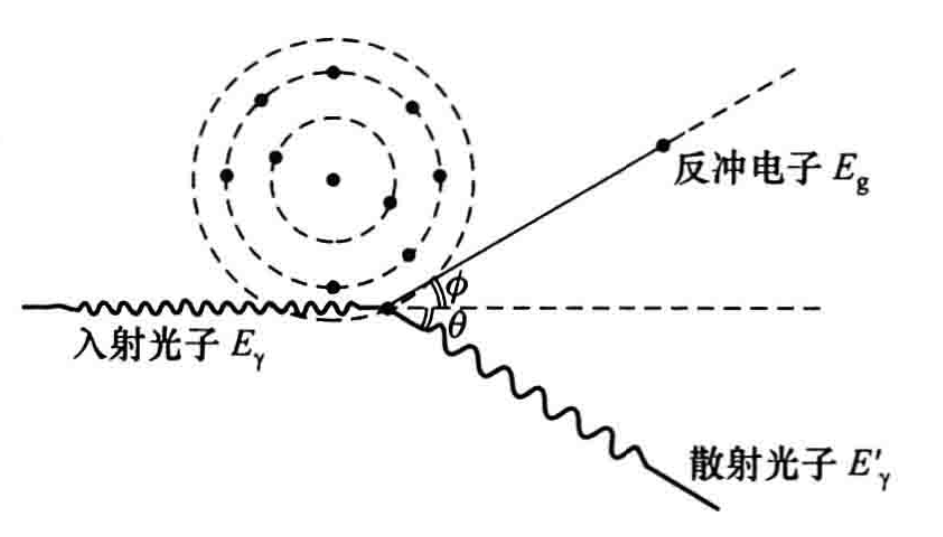
\includegraphics[width=0.85\linewidth]{fig/lilun.png}
  \caption{康普顿散射实验示意图}
  \label{fig:lilun}
\end{figure}
  
康普顿散射的微分界面满足克莱因-仁科公式:
$$ 
\frac{\mathrm{d}\sigma(\theta)}{\mathrm{d}\Omega} = r_0^2 \left[ \frac{1}{1 + \alpha(1 - \cos\theta)} \right]^2 \left[ \frac{1 + \cos^2\theta}{2} \right] \left[ 1 + \frac{\alpha^2(1 - \cos\theta)^2}{(1 + \cos^2\theta)\left[ 1 + \alpha(1 - \cos\theta) \right]} \right]
$$
本实验所测得的微分散射截面的相对值$\frac{d\sigma(\theta)}{d\Omega}/\frac{d\sigma(\theta_0)}{d\Omega}$满足:
$$
\frac{\mathrm{d}\sigma(\theta)}{\mathrm{d}\Omega} \bigg/ \frac{\mathrm{d}\sigma(\theta_0)}{\mathrm{d}\Omega} = \frac{N_{\mathrm{p}}(\theta)}{R(\theta)\eta(\theta)} \bigg/ \frac{N_{\mathrm{p}}(\theta_0)}{R(\theta_0)\eta(\theta_0)}
$$
其中,$N_{\mathrm{p}}(\theta)$可以由实验测量得到,
而$R(\theta)$和$\eta(\theta)$可以由教材\cite{jindaiwulishiyan}中给出的表格中的数值再经过三次样条插值得到,分别如\autoref{fig:R}和\autoref{fig:eta}所示。

\begin{figure}[htbp]
  \centering
  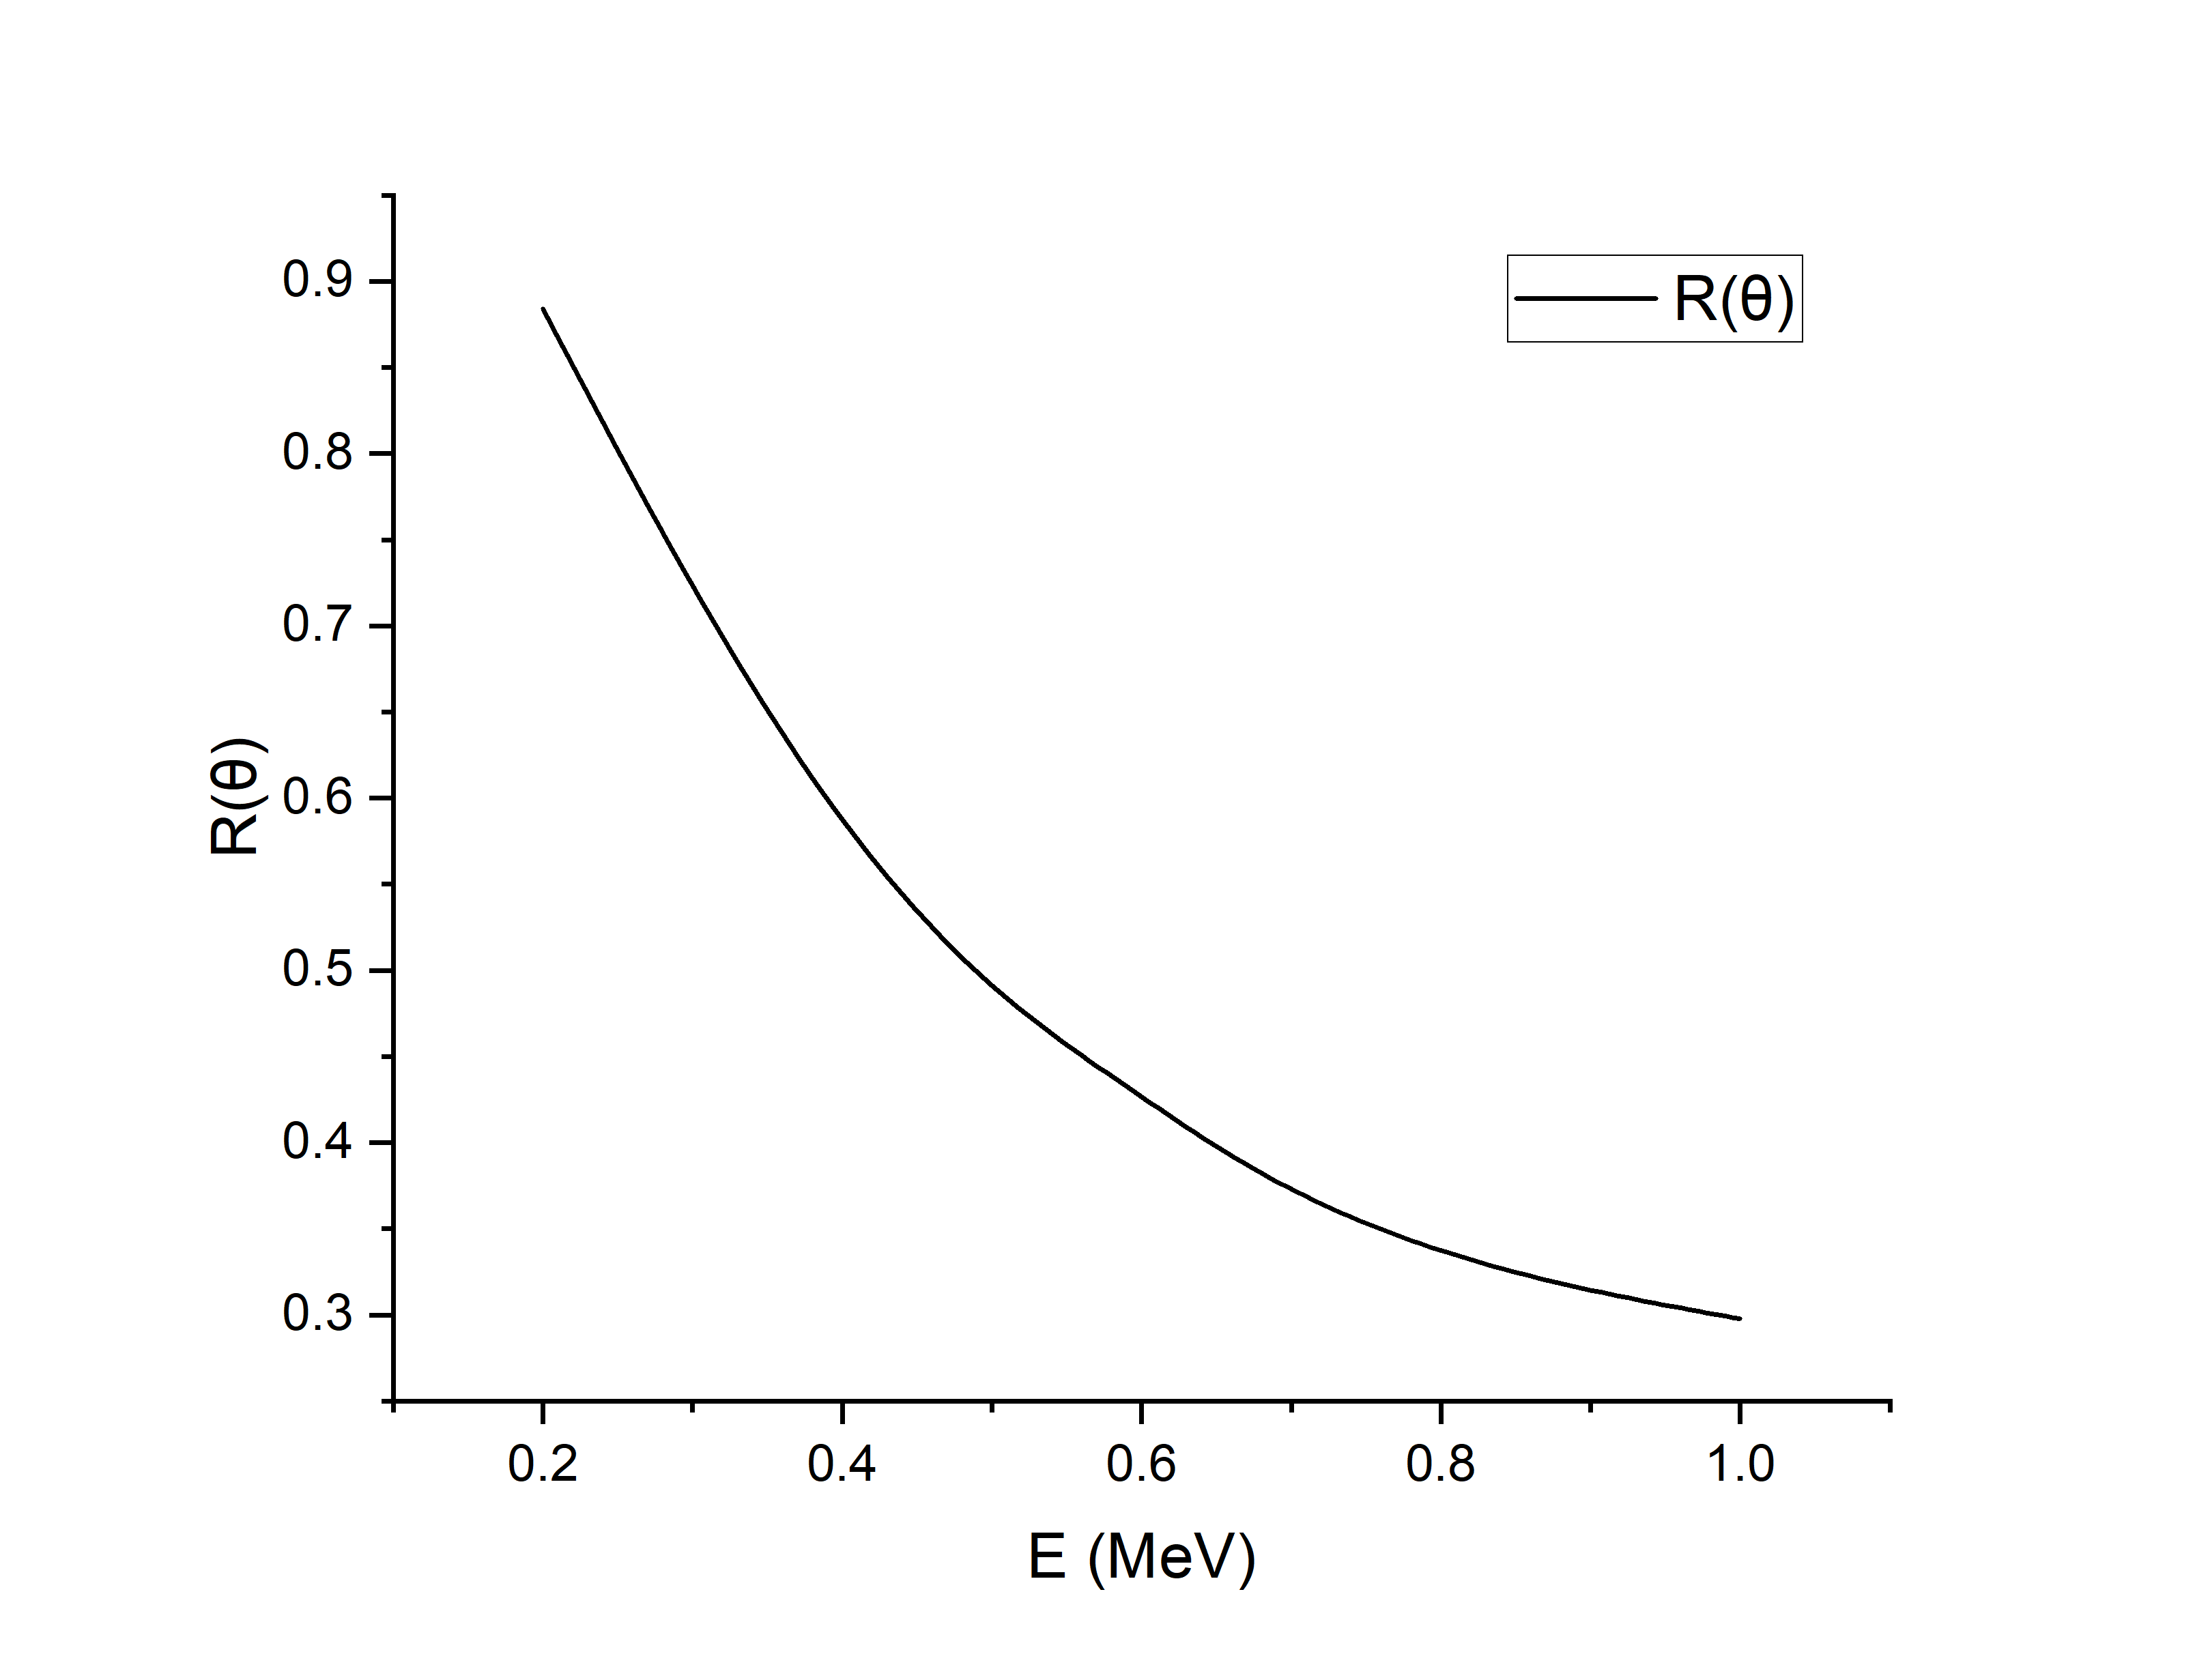
\includegraphics[width=0.85\linewidth]{fig/R.png}
  \caption{$R(\theta)$}
  \label{fig:R}
\end{figure}

\begin{figure}[htbp]
  \centering
  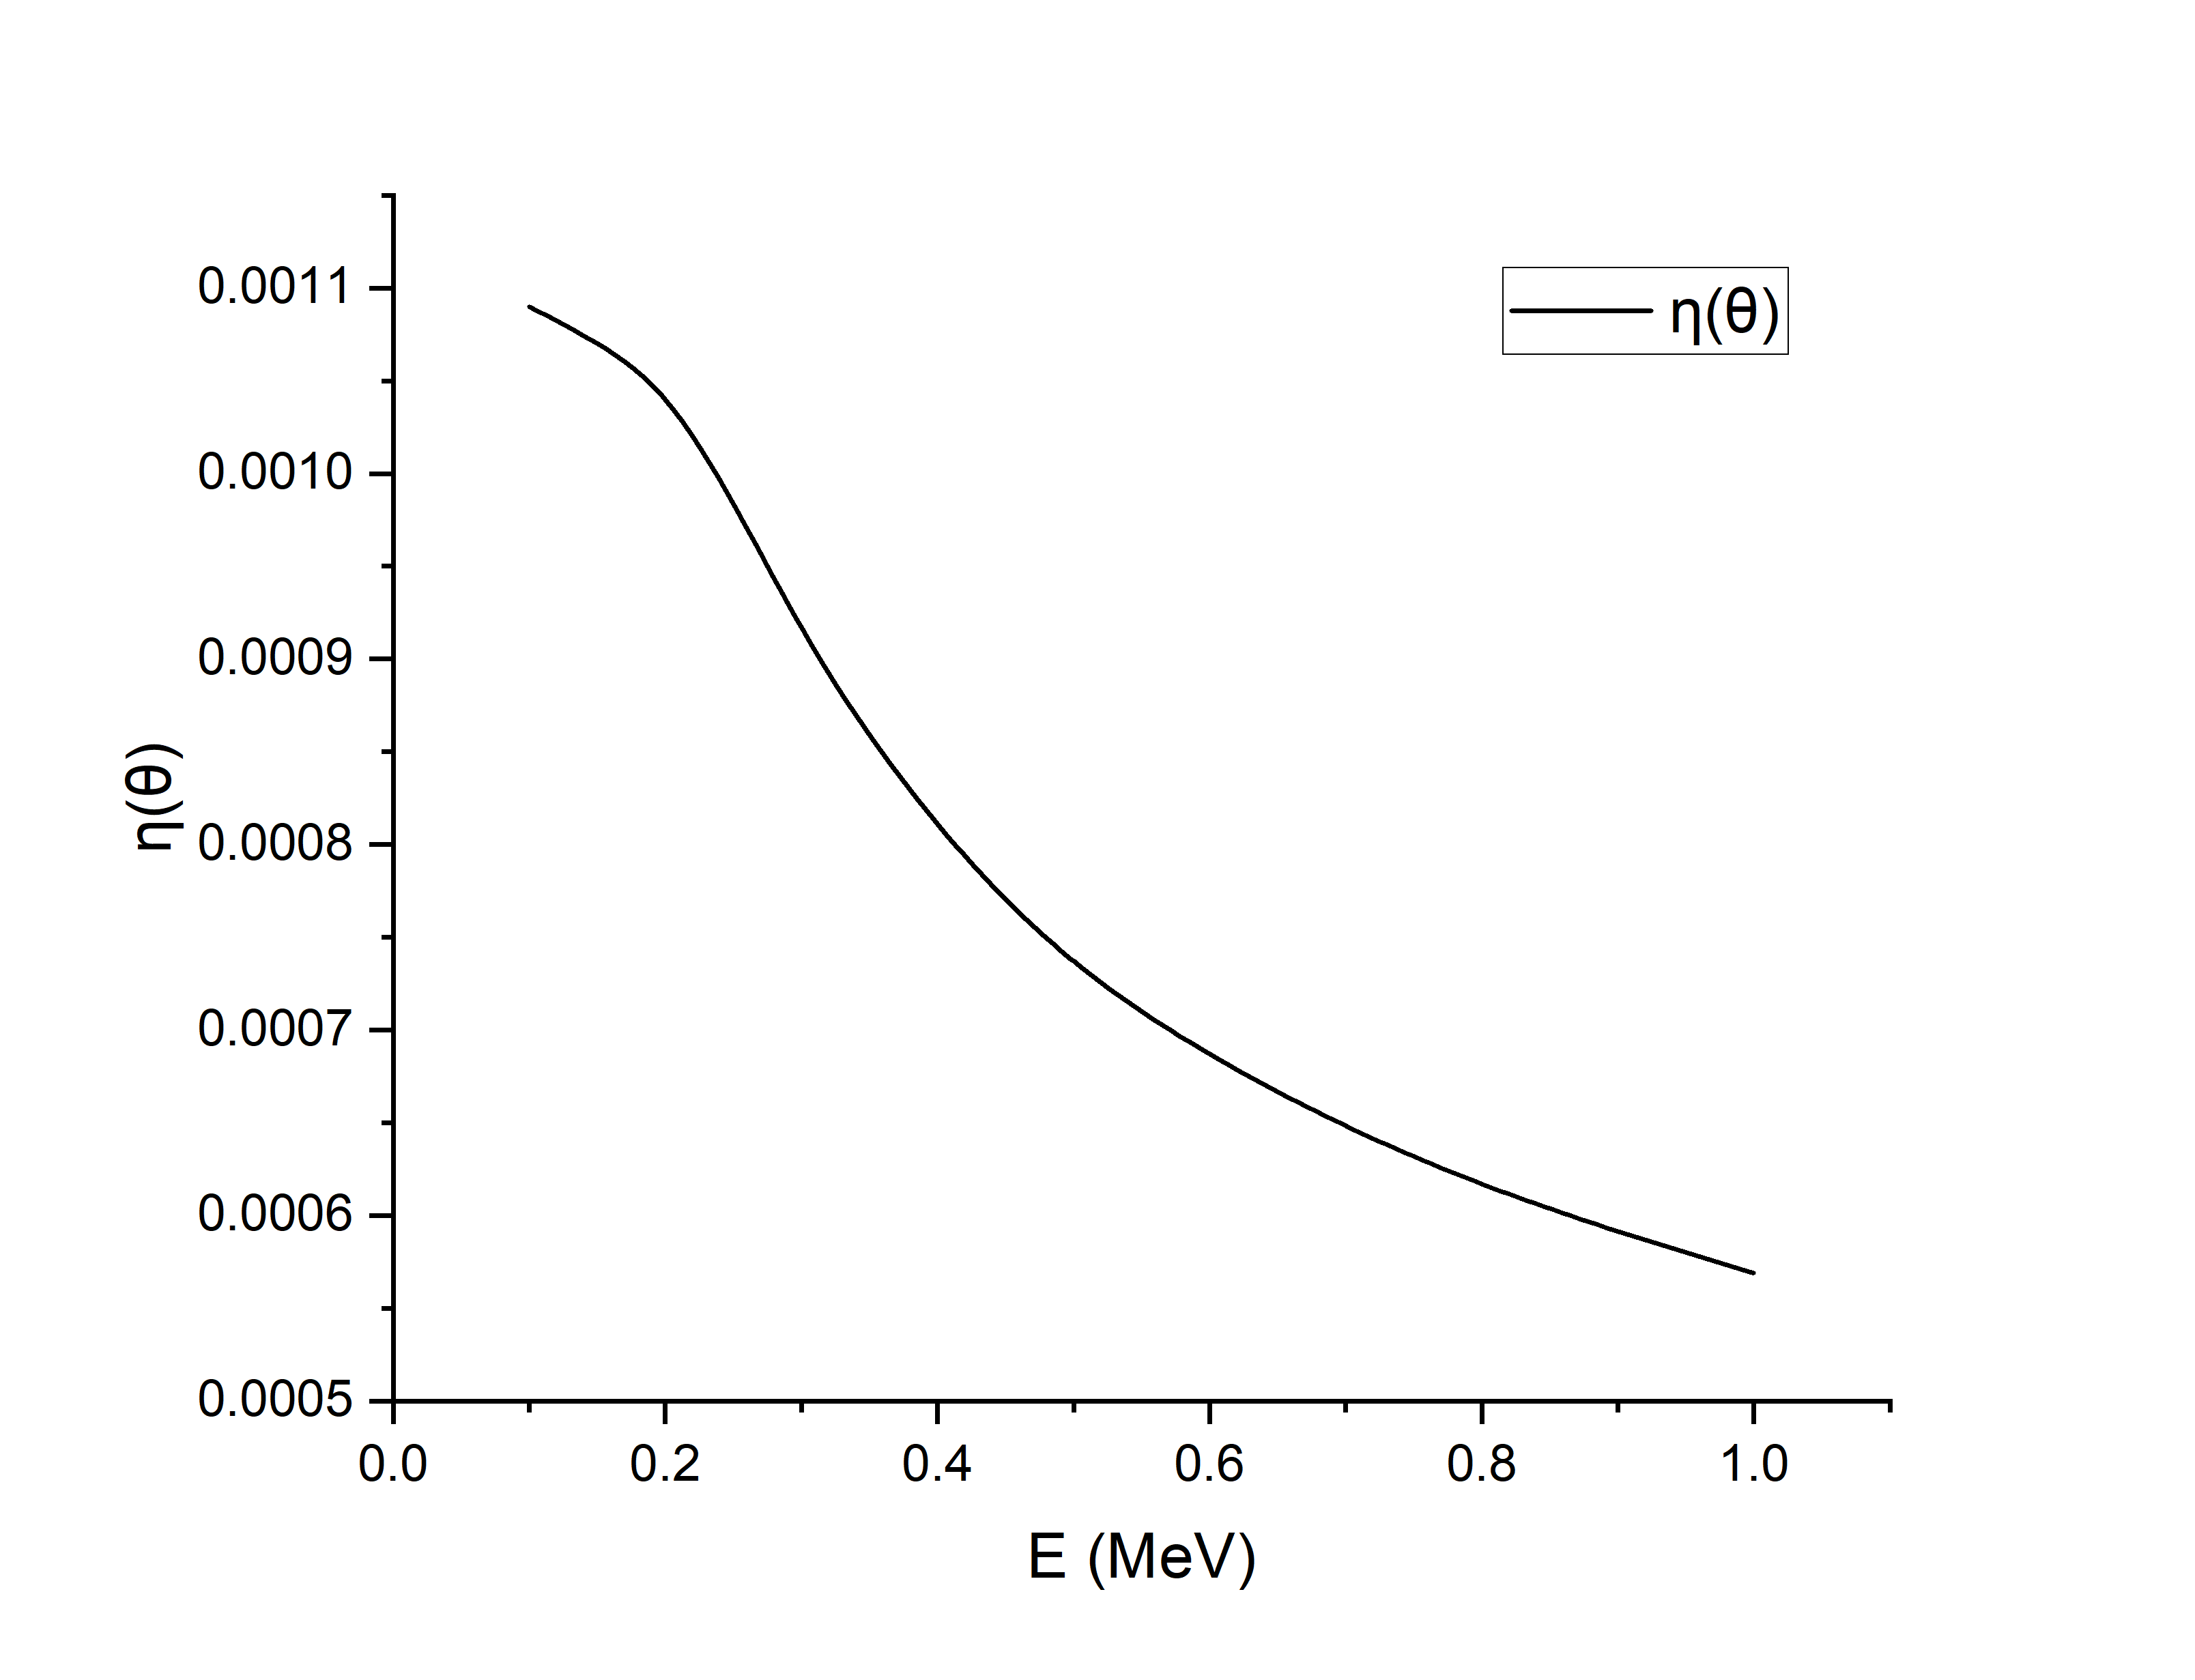
\includegraphics[width=0.85\linewidth]{fig/yita.png}
  \caption{$\eta(\theta)$}
  \label{fig:eta}
\end{figure}

\section{实验}
\subsection{实验装置示意}
实验装置如\autoref{fig:zhaungzhi}所示。

\begin{figure}[htbp]
  \centering
  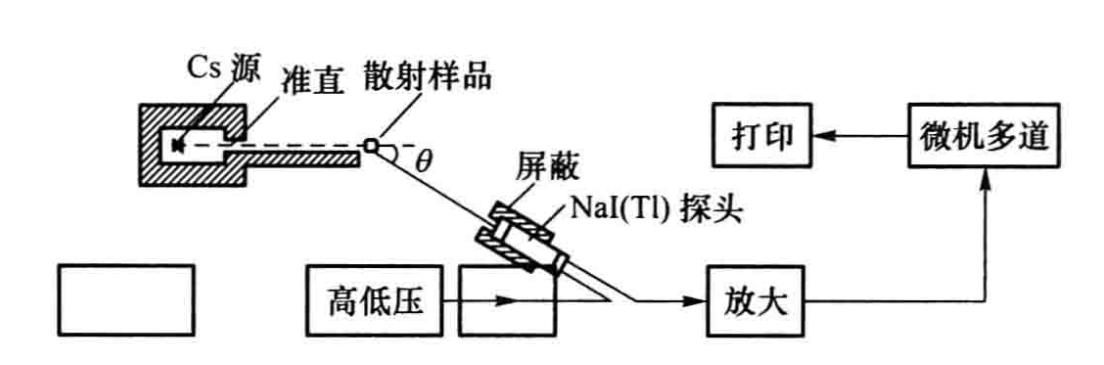
\includegraphics[width=0.85\linewidth]{fig/zhuangzhi.png}
  \caption{康普顿散射实验装置示意图}
  \label{fig:zhaungzhi}
\end{figure}


\subsection{实验步骤}
  \subsubsection{标定能量刻度}
    \begin{enumerate}
      \item 打开${^{137}Cs}$源,将开关打在半开状态,取下散射棒. 调节探头高压$\text{HV=520V}$,预热10分钟. 调节放大$\text{GAIN ADJ} = 3.8$,使得$0.662\text{MeV}$光电峰落在480道左右. 测量其全能谱,通过寻峰定出全能峰对应的准确道数.
      \item 关闭${^{137}Cs}$源,放上${^{60}Co}$,测量其全能谱,定出$1.17\text{MeV}$和$1.33\text{MeV}$两峰对应的准确道数.
      \item 根据测得的三个峰的道址,利用最小二乘法做能量刻度。
    \end{enumerate}

  \subsubsection{康普顿散射峰值和微分截面测量}
    \begin{enumerate}
      \item 安装散射棒,完全打开${^{137}Cs}$源,测量微分散射截面和散射峰能量随散射角的变化. 散射
      角分别取$\theta = 20^\circ,40^\circ ,60^\circ ,80^\circ ,100^\circ ,120^\circ $,对于每个散射角,利用操作
      “寻峰”和“重点区计算”,找出并记录下光电峰的峰位、左右光标道址、重点区总面积. 
      \item 取下散射棒,记录和有散射棒时相同道数区间的面积总计数,从而计算出净峰面积.
      \item 计算散射$\gamma$光子能量和微分散射截面与散射角$\theta$的关系,画出相应关系曲线图,
      并计算实验值和理论值的偏差.在计算过程中,探测器的$R(E), \eta(E)$由 Origin 三次样条插值得到.
    \end{enumerate}

\section{结果及讨论}

  \subsection{实验结果}

    测量${^{137}Cs}$的全谱,通过寻峰定出全能峰对应的道数为 468 . 接着测量${^{60}Co}$的全谱,定出$1.17\text{MeV}$和$1.33\text{MeV}$的对应的道数为$848$和$955$.
    对能量$E$和道数$d$进行最小二乘法拟合$E = a \cdot d + b $,拟合的相关系数为$r = 0.9978$,拟合参数为:
    $$a = 1.36 \times 10^{-3}, \quad b = 2.261 \times 10^{-2}$$

    \begin{figure}[htbp]
      \centering
      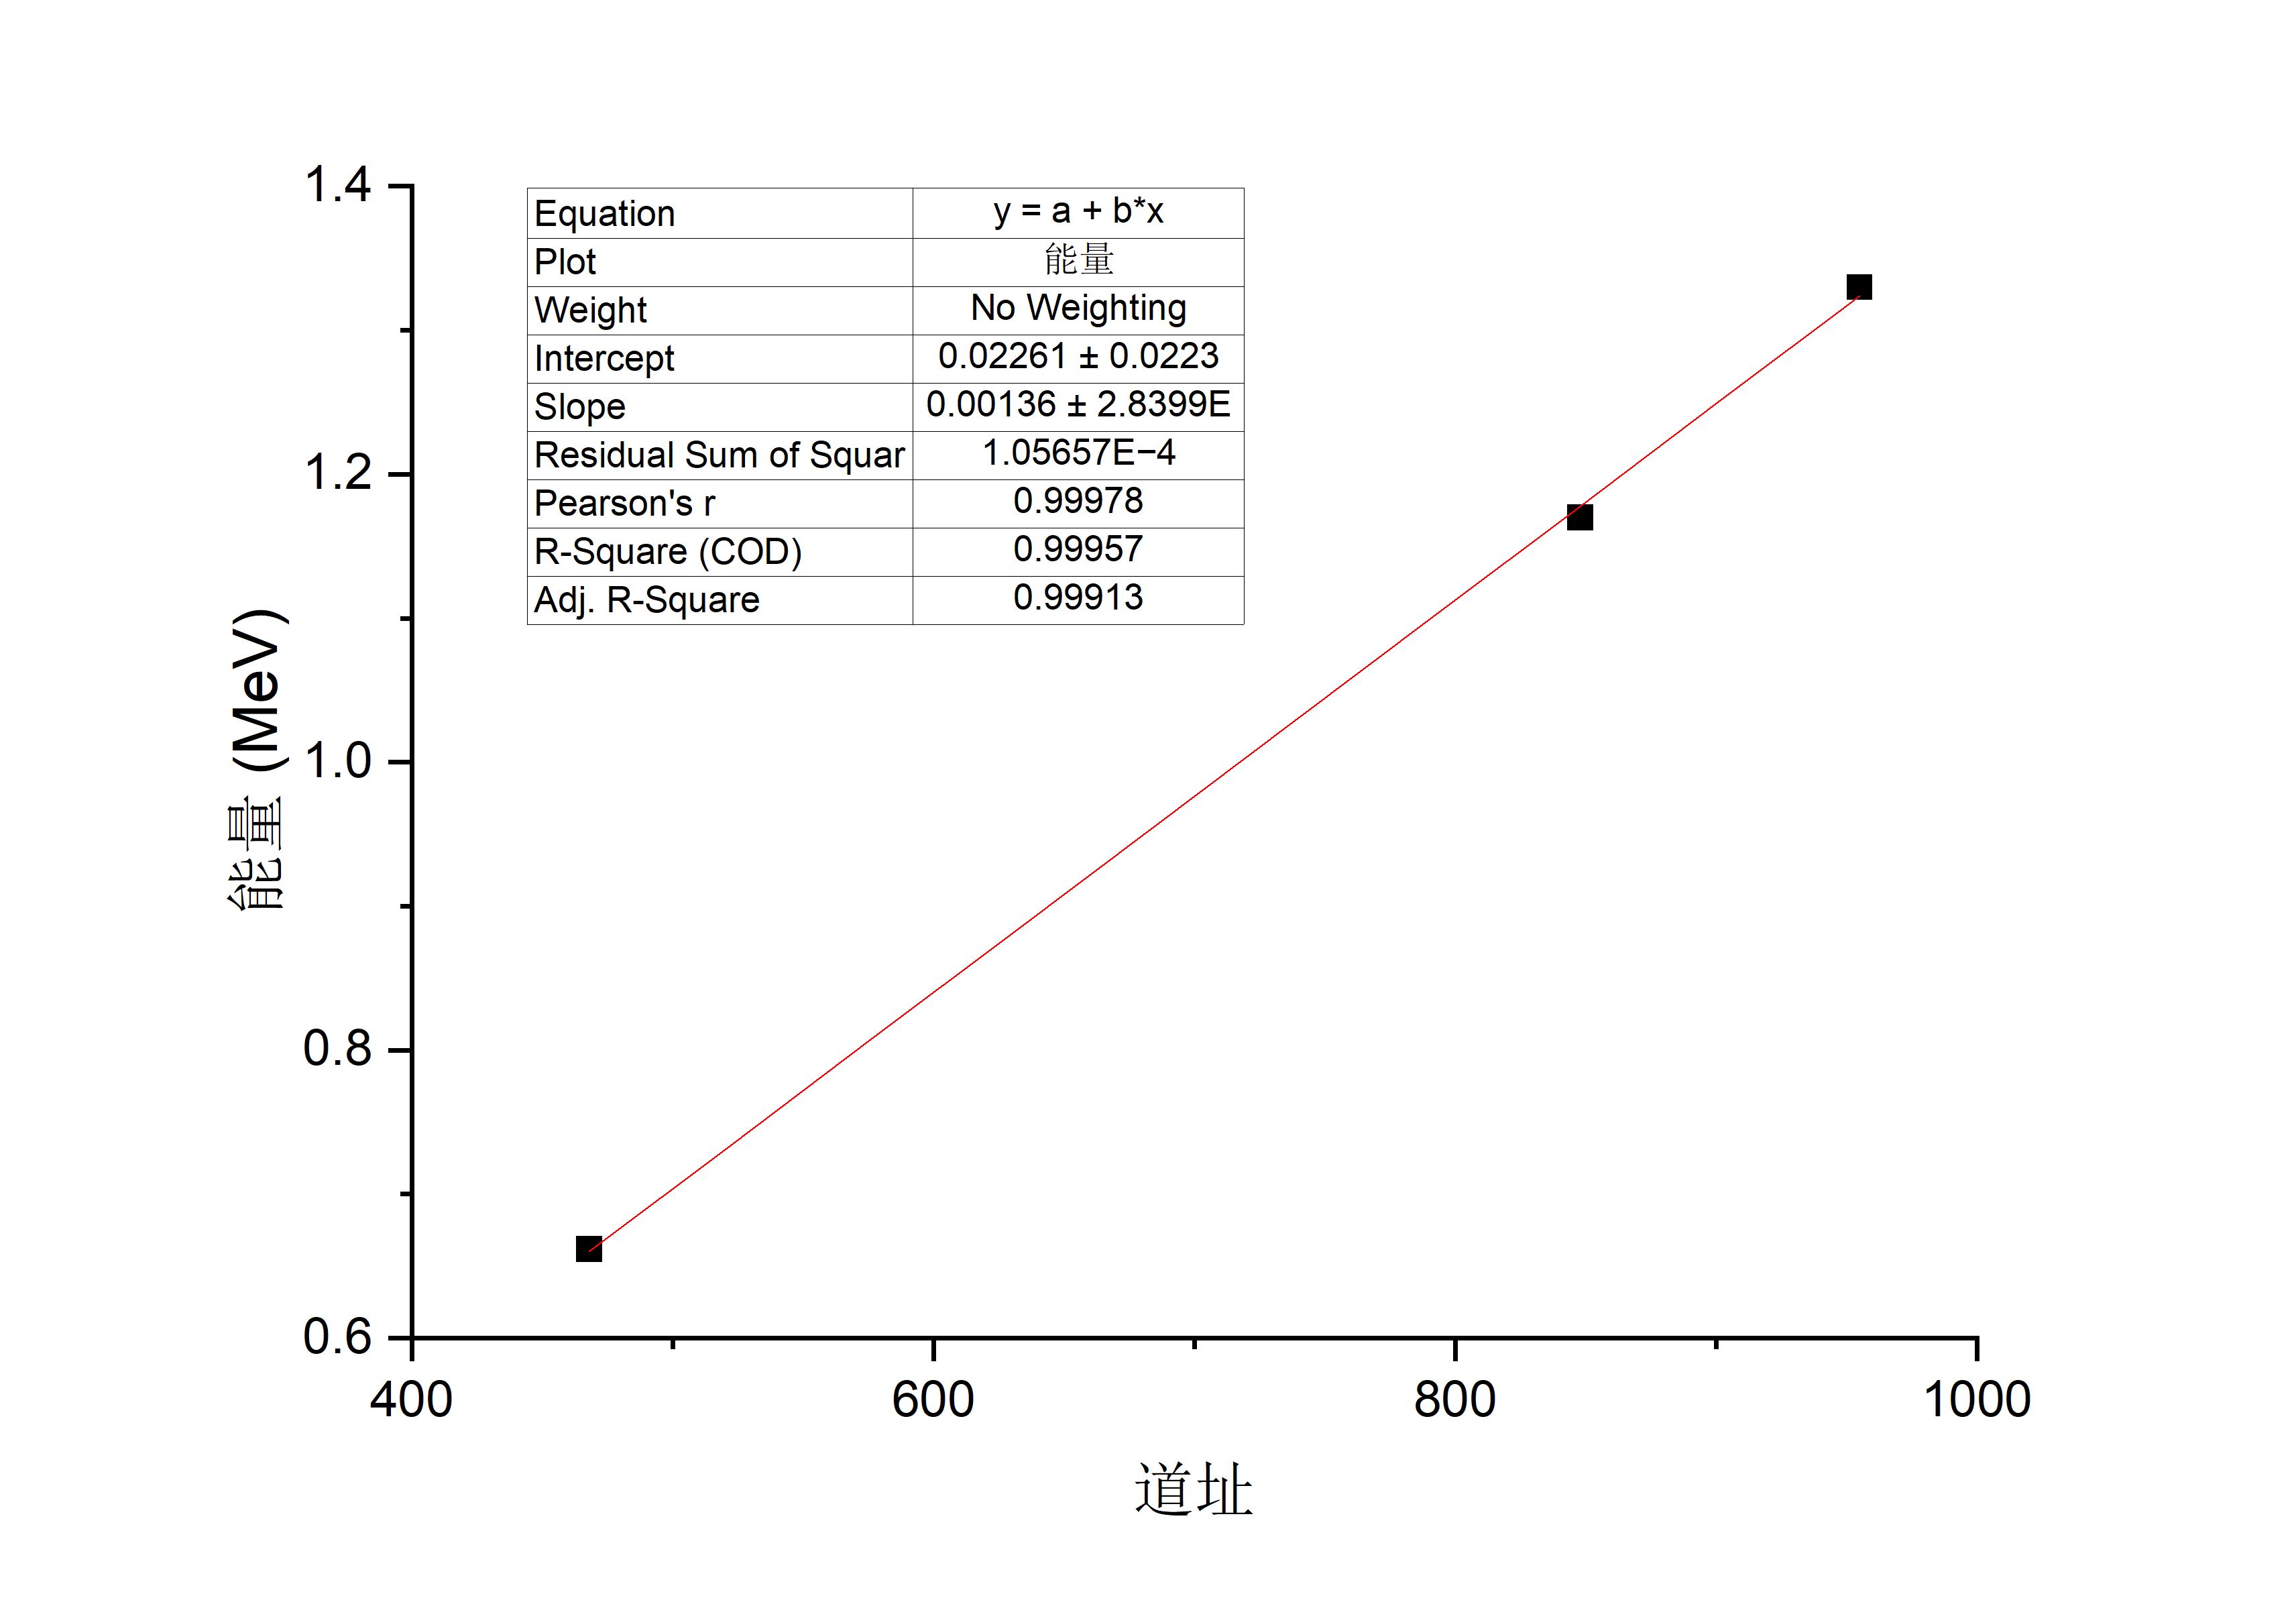
\includegraphics[width=0.85\linewidth]{fig/nihe.png}
      \caption{能量-道址线性刻度}
      \label{fig:nihe}
    \end{figure}

    \subsection{康普顿散射峰值和微分截面测量}

    改变散射角分别对散射信号和本底信号进行测量, 得到的测量结果如\autoref{jiaodu}所示,它是散射信号减去本地信号的画图结果。
    
    得到的结果如\autoref{}所示.

      \begin{figure}[htbp]
        \centering
        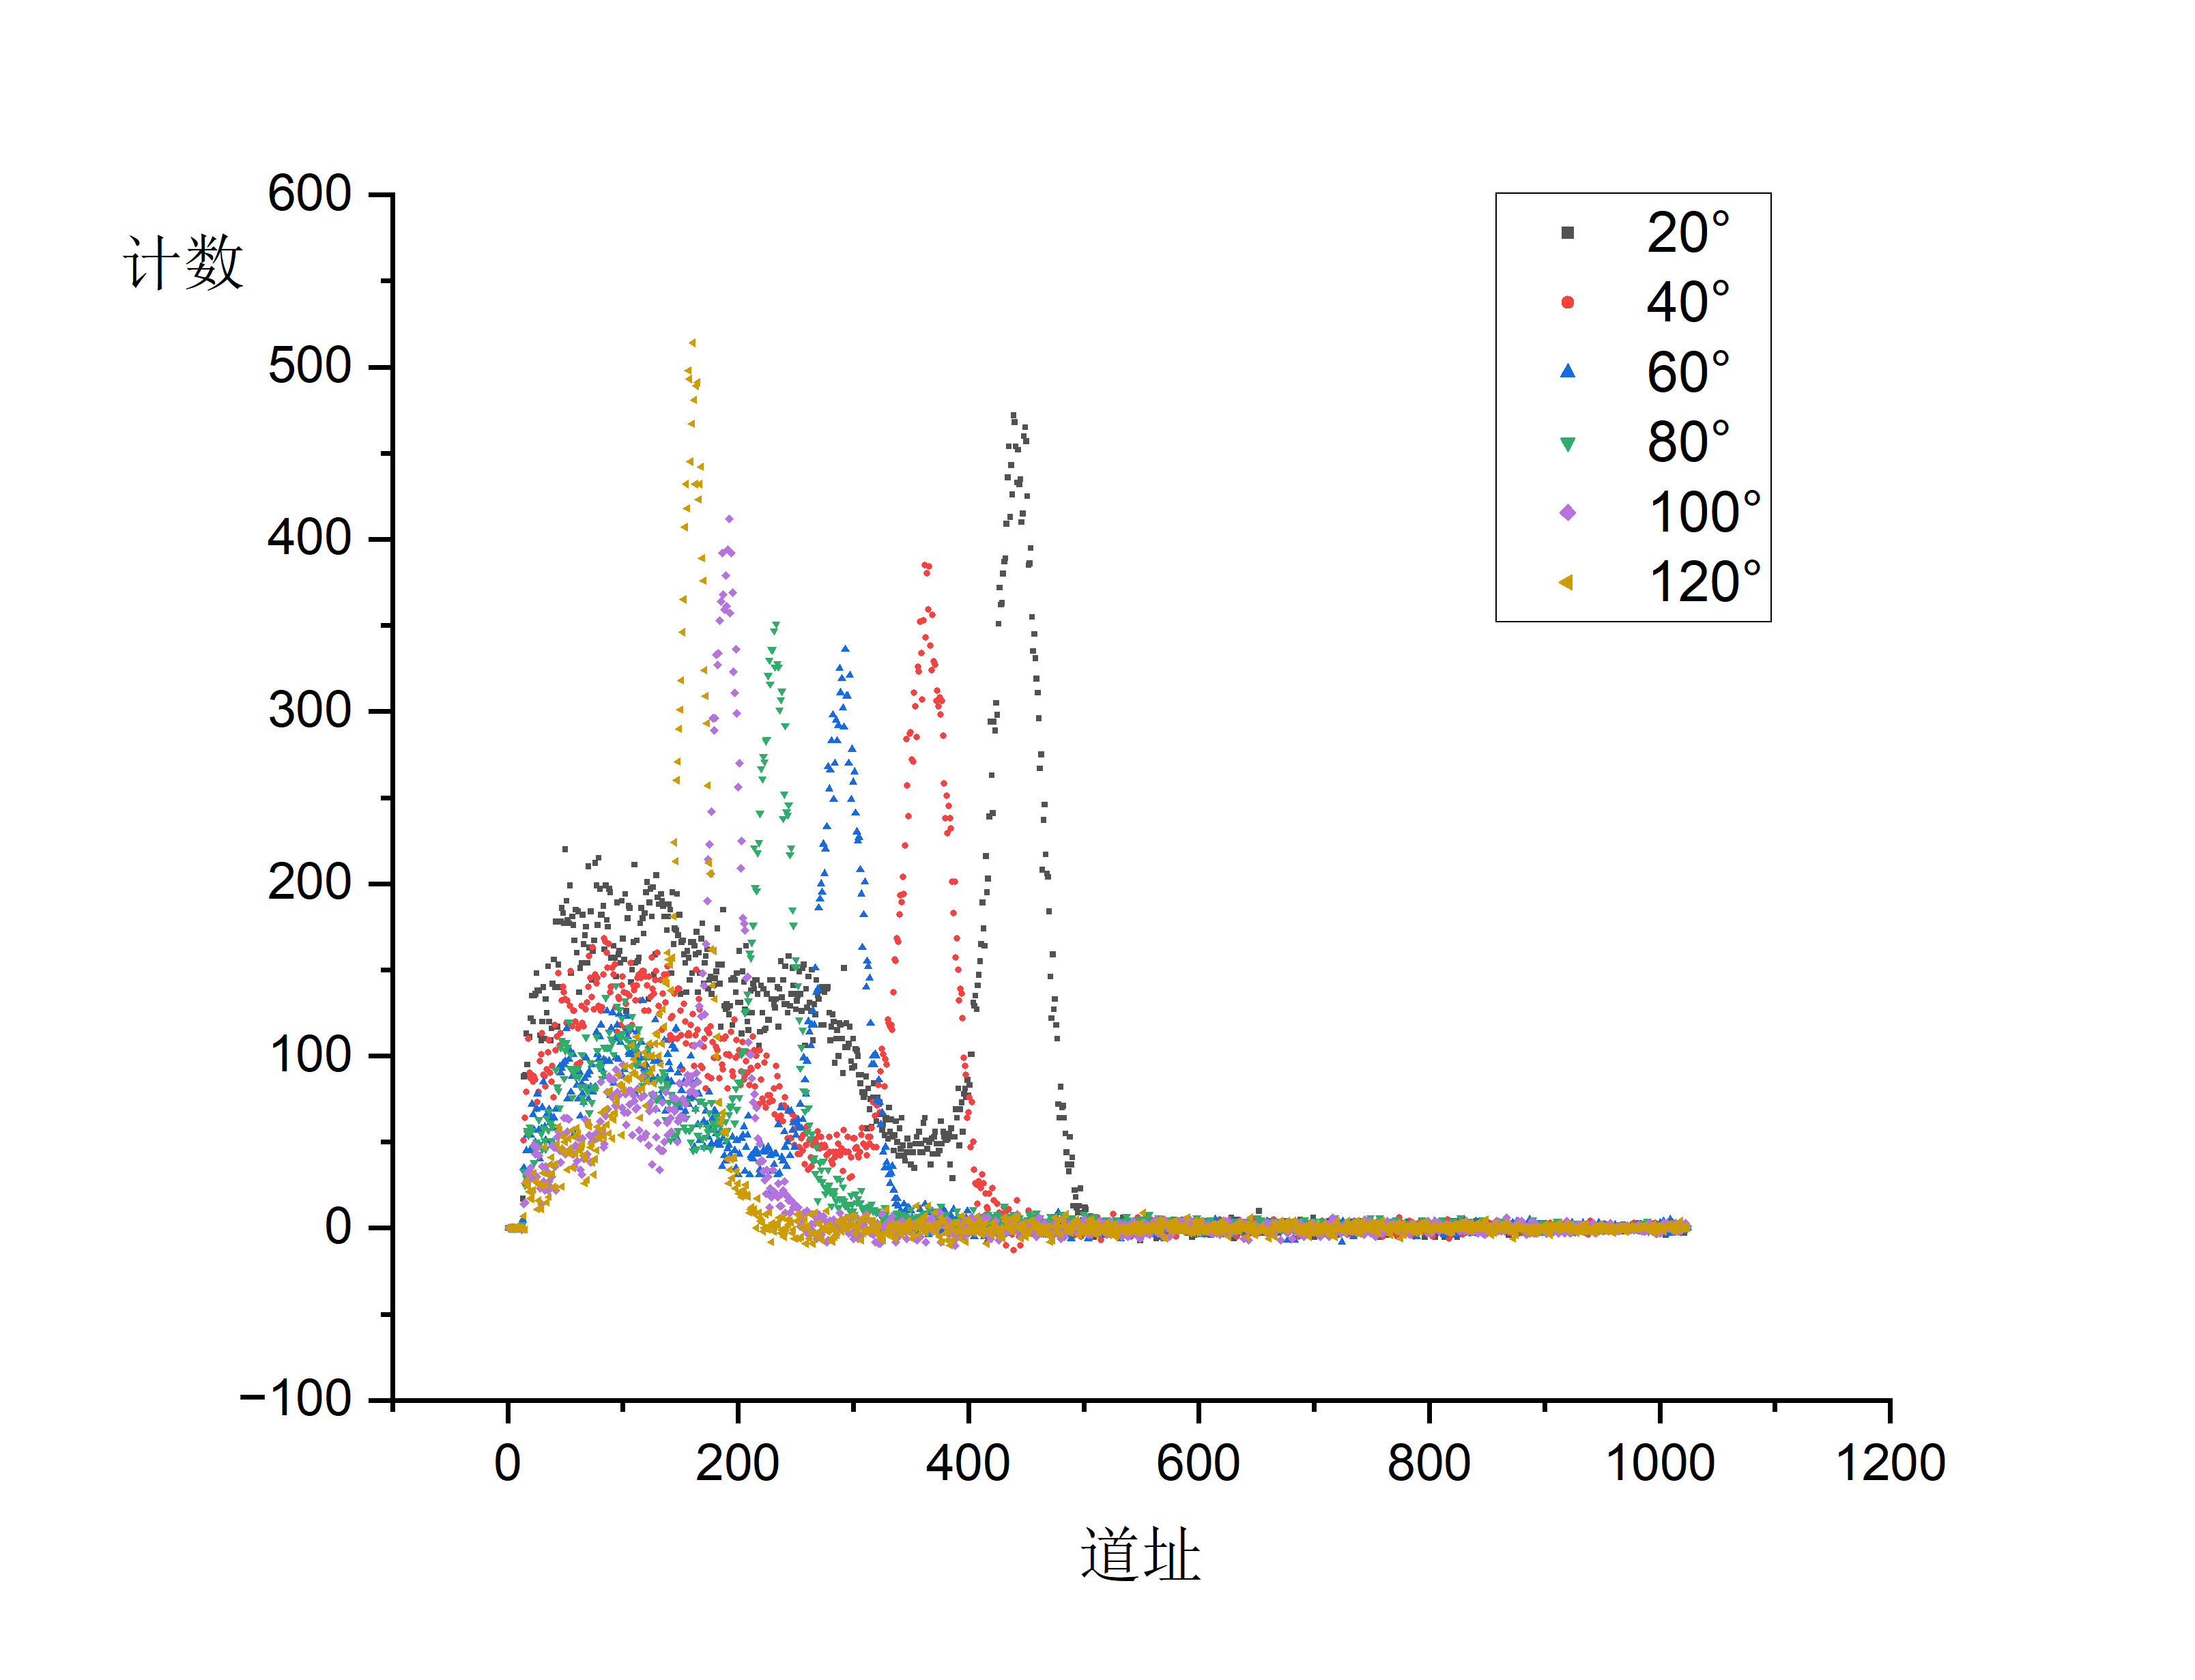
\includegraphics[width=0.85\linewidth]{fig/jiaodu.png}
        \caption{不同角度处的散射能谱}
        \label{fig:jiaodu}
      \end{figure}

      \begin{table}[htbp]
        \centering
        \caption{散射γ光子能量测量与理论对比数据} % 表格标题(可根据实际需求修改)
        \begin{tabular}{ccccccc}
            \toprule % 顶部粗线(需加载booktabs宏包)
            散射角 $\theta$ ($^\circ$) & 峰位道址 & 能量实验值 (MeV) & $R(\theta)$ & $\eta(\theta)$ & 能量理论值 (MeV) & 能量偏差 (\%) \\
            \midrule % 中间细线(需加载booktabs宏包)
            20 & 447 & 0.63053 & 0.409 & 0.000674 & 0.613735 & 2.66 \\
            40 & 361 & 0.51357 & 0.481 & 0.000729 & 0.507823 & 1.12 \\
            60 & 292 & 0.41973 & 0.565 & 0.000794 & 0.401635 & 4.31 \\
            80 & 232 & 0.33813 & 0.669 & 0.000872 & 0.319645 & 5.47 \\
            100 & 191 & 0.28237 & 0.751 & 0.000940 & 0.262597 & 7.00 \\
            120 & 160 & 0.24021 & 0.818 & 0.000996 & 0.224898 & 6.37 \\
            \bottomrule % 底部粗线(需加载booktabs宏包)
        \end{tabular}
        \label{tab:gamma_scattering_energy} % 表格引用标签(方便文中引用)
      \end{table}




  无磁场 (I = 0 A) 下汞灯的光谱如\autoref{fig:000}所示. 在一个光谱周期内, 仅存在一个 546.1 nm 的主峰. 其余的少量突起可能是精细结构的体现.
  \par
  磁场为 0.8 T (I = 4 A) 下汞灯的子谱线如\autoref{fig:444}所示, 磁场为 1.0 T (I = 5 A) 下汞灯的子谱线如\autoref{fig:555}所示. 
  相对于\autoref{fig:000}来说, 加磁场后谱线发生了分裂, 在一个光谱周期内原来的 546.1 nm 线分裂成了 9 条子谱线, 
  并且电流越大, 磁场越大, 谱线分裂得越明显. 

  在光路中加入偏振片, 旋转偏振片的角度, 在两个相互垂直的方向可以测得 $\pi$ 线和 $\sigma$ 线, 分别如\autoref{fig:551}和\autoref{fig:552}所示.
  可以看到, \autoref{fig:551}中在一个周期保留的三条线是 \pi 线, 
  而\autoref{fig:552}中在一个周期保留的六条线是$\sigma$线, 这和我们的理论分析\autoref{fig:lilun}一致.
  图中的杂峰没能被滤去可能是由于偏振片方向放置放的不够正确导致的.

\begin{figure}[htbp]
  \centering
  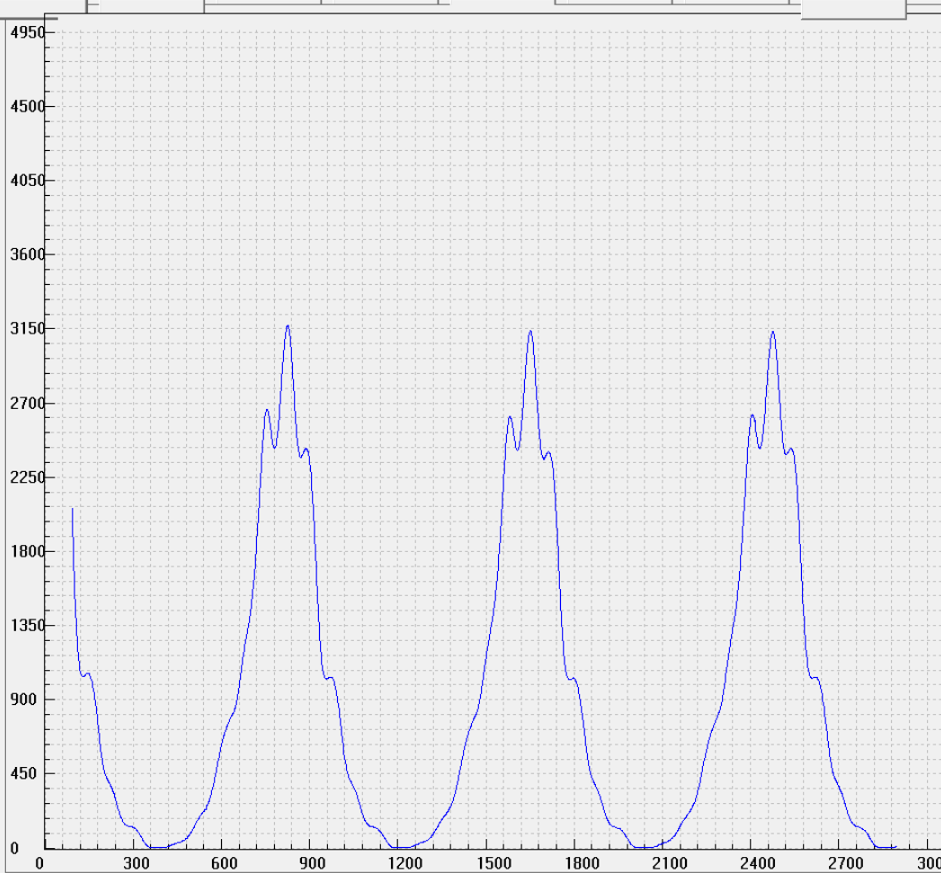
\includegraphics[width=0.85\linewidth]{fig/3.png}
  \caption{磁场为 1.0 T (I = 5 A) 下汞灯的 \pi 线}
  \label{fig:551}
\end{figure}
\begin{figure}[htbp]
  \centering
  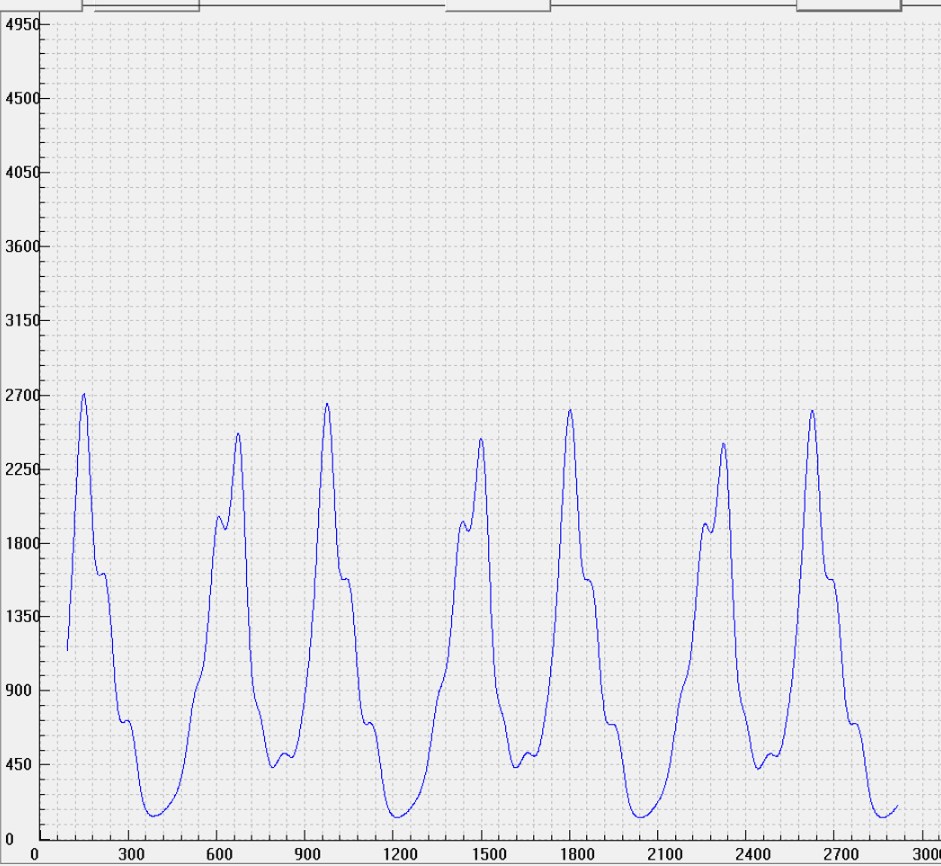
\includegraphics[width=0.85\linewidth]{fig/4.png}
  \caption{磁场为 1.0 T (I = 5 A) 下汞灯的 $\sigma$ 线}
  \label{fig:552}
\end{figure}

\subsection{各子谱线的波数差偏移和强度}

在\autoref{fig:555}中, 分裂谱线相对于主谱线的裂距和相对强度列表分别如\autoref{tab:liejv}和\autoref{tab:qiangdu}所示,
通过实验数据可以计算得出, 对于波数差$\delta \nu_R = 2.5 cm^{-1}$, 对应的压强差为 825.25 arb.units.


\begin{table}[htbp]
  \centering
  \caption{外磁场为 1.0 T 情形下, 各子谱线相对于 546.1 nm 谱线的波数差偏移}
  \begin{tabular}{c|ccccccccc}
    \hline
    n 峰 & -4 & -3 & -2 & -1 & 0 & 1 & 2 & 3 & 4 \\
    \hline
    $\Delta p$ & -284.667 & -211.667 & -148.333 & -74 & 0 & 73 & 148.667 & 216.333 & 290.333 \\
    \hline
    $\Delta \nu_{\text{exp}} (cm^{-1})$ & -0.862 & -0.641 & -0.449 & -0.224 & 0 & 0.221 & 0.450 & 0.655 & 0.880 \\
    \hline
    $\Delta \nu_{\text{theo}} (cm^{-1})$ & -0.934 & -0.701 & -0.467 & -0.234 & 0 & 0.234 & 0.467 & 0.701 & 0.934 \\
    \hline
  \end{tabular}
  \label{tab:liejv}
\end{table}

\begin{table}[htbp]
  \centering
  \caption{各子谱线的强度对比}
  \begin{tabular}{c|ccccccccc}
    \hline
    n 峰 & -4 & -3 & -2 & -1 & 0 & 1 & 2 & 3 & 4 \\
    \hline
    绝对强度 & 1012.667 & 2157.333 & 2930.667 & 2901.333 & 3237.333 & 2788 & 2961.333 & 1635.333 & 733.333 \\
    \hline
    相对强度 & 1.251 & 2.666 & 3.621 & 3.585 & 4 & 3.445 & 3.659 & 2.021 & 0.906 \\
    \hline
    相对强度理 & 0.500 & 1.500 & 3 & 3 & 4 & 3 & 3 & 1.500 & 0.500 \\
    \hline
  \end{tabular}
  \label{tab:qiangdu}
\end{table}

根据\autoref{tab:liejv}可以发现, 外磁场为 1.0 T 情形下, 
实验测得的各子谱线相对于 546.1 nm 谱线的波数差偏移与理论值比较符合, 不过所有的实验得到的波数差偏移绝对值均小于理论值.
造成这一现象的可能原因有:
\begin{itemize}
  \item 洛伦兹单位$\tilde{L} = \frac{eB}{4\pi mc} \approx 0.467B$, 但实验实际的磁场大小比理论的 1.0 T 要小.
  \item 原子内部精细结构的影响.
\end{itemize}

而分析\autoref{tab:qiangdu}会发现, 实验测得的相对强度比理论得到的大许多, 并且强度呈现左右不对称的情况. 
在左侧编号为 -4 和 -3 的峰的高度比与其对称的右侧编号为 4 和 3 的峰的高度要高很多.
造成这一现象的可能原因有:
\begin{itemize}
  \item 精细结构的影响.
  \item 实验过程中磁场与成像设备和标准具所在的直线并不垂直. 因此测量得到的谱线分裂情况并不具有各向同性, 也因此强度不对称.
  \item 分裂得到的子谱线之间挨得很近, 彼此之间会产生影响, 导致测量得到的谱线强度并不是真实的谱线强度.
\end{itemize}

\subsection{荷质比的计算}

洛伦兹单位的表达式是$$ \tilde{L} = \frac{eB}{4\pi mc}$$
从而可以得到荷质比的表达式$$\frac{e}{m} = \frac{4\pi c \tilde{L}}{B}$$

洛伦兹单位 L 的值可以由线性拟合算出. 根据\autoref{tab:liejv}的峰的变好和裂距的实验测得值, 得到如\autoref{222}所示的直线.
\begin{figure}[htbp]
  \centering
  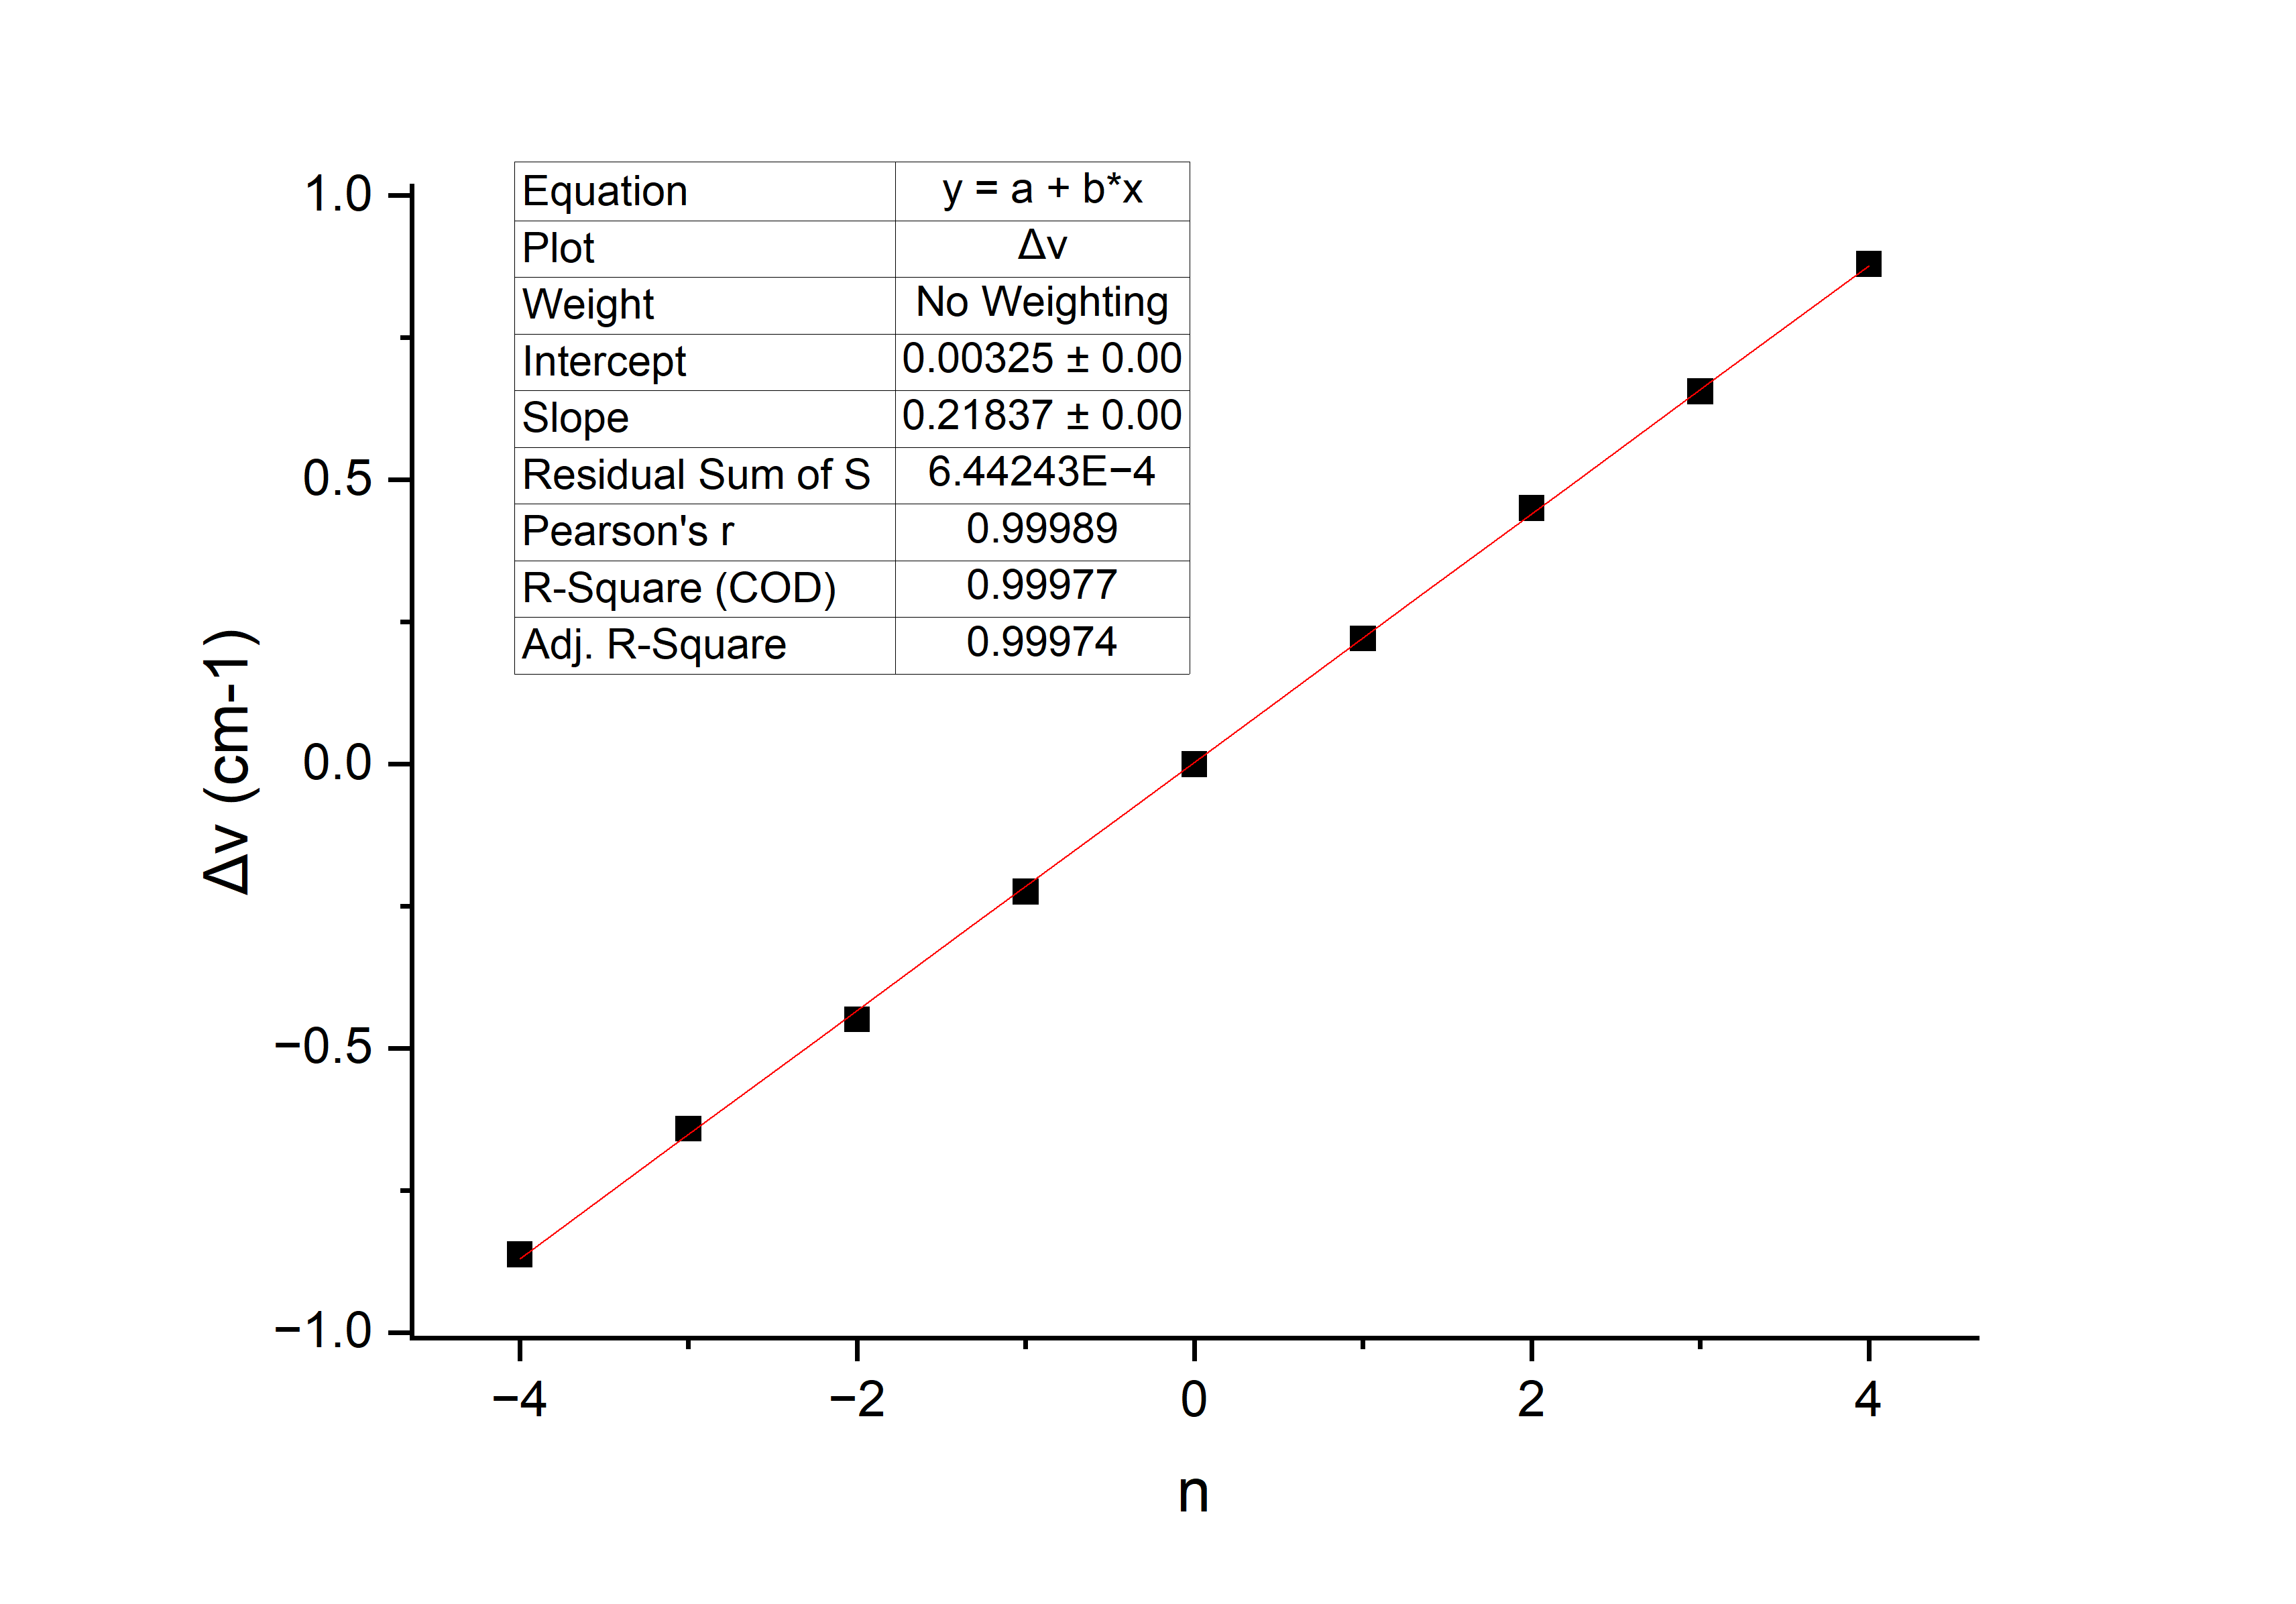
\includegraphics[width=0.85\linewidth]{fig/222.png}
  \caption{\delta \nu 与 n 的关系}
  \label{fig:222}
\end{figure}

拟合得到的斜率$$k = 0.21837 cm^{-1}$$
于是可以计算得到$$ \tilde{L} = 2k = 0.43674 cm^{-1}$$
带入磁场的大小 B = 1.0 T, 从而可以计算得到荷质比为$$\frac{e}{m} = \frac{4\pi c \tilde{L}}{B} = 1.65 \times 10^{11} C/kg$$
而查资料可知, 电子的比荷为$1.76 \times 10^{11} C/kg$, 相对误差为$ 6.25\%$. 这里误差产生的可能原因有:
\begin{itemize}
  \item 实验中实际的磁场大小不等于 1.0 T, 导致带入荷质比表达式中的 B 不准确.
  \item 在之前的讨论中有发现, 实验测得的峰与峰之间的裂距普遍比理论值小, 这会导致拟合得到的斜率偏小, 从而导致洛伦兹单位偏小, 从而使得计算得到的荷质比偏小.
\end{itemize}

 
\section{结论}
  本实验借助气压扫描式 F-P 标准具, 
  对汞灯 546.1 nm 谱线及其在磁场作用下的塞曼光谱进行观察与测量.
  报告呈现了该谱线在无磁场、0.8 T 磁场 (4 A 励磁电流) 及 1.0 T 磁场 (5 A 励磁电流) 下的光谱图, 
  同时得到了 1.0 T 磁场中 $\pi$ 线和 $\sigma$ 线的光谱. 
  本研究确定了 1.0 T磁场下各子谱线相对于 546.1 nm 谱线的波数差及相对强度, 
  并通过列表与理论值对比, 讨论了产生误差的原因.
  此外, 本研究还对各子谱线波数差进行拟合计算, 得到电子荷质比实验值$1.65 \times 10^{11} C/kg$, 并将其和理论值相比较, 分析了误差产生的原因.

\begin{acknowledgments}
  感谢洪浩老师和助教老师的耐心指导和帮助.
  \par
  感谢搭档王尉丞同学的协助.
\end{acknowledgments}

% bibliography 的参数是你的 *.bib 文件去掉后缀名后的部分
\bibliography{bibli}

\clearpage % 附录前另起一页
\appendix % 附录开始
\section{思考题}\label{app:exercise}
\subsection{从塞曼分裂谱中如何确定能级的 J 量子数?}
要确定能级的 $J$ 量子数, 可以利用塞曼分裂中 $\pi$ 线与 $\sigma$ 线的数目进行推断, 其逻辑如下:
首先, $\pi$ 线对应磁量子数满足 $\Delta M_J = 0$ 的跃迁. 
观测到的 $\pi$ 线数量反映了上下两个能级间相同磁量子数取值的重合情况. 
举例来说, 若出现 3 条 $\pi$ 线, 说明两个能级中有 3 个相同的磁量子数 (如 $M_J = -1, 0, 1$) . 
其次, $\sigma$ 线对应 $\Delta M_J = \pm 1$ 的跃迁. 
观测到 6 条 $\sigma$ 线, 意味着其中一个能级的磁量子数可取值为 $M_J = -2, -1, 0, 1, 2$, 即比另一个能级多出两个取值. 
结合 $\pi$ 线和 $\sigma$ 线的数目, 
可以推断出两个能级的总角动量量子数分别为 $J = 1$ 和 $J = 2$. 
\subsection{根据塞曼分裂谱的裂距如何确定能级的 g 因子数?}
根据公式$\Delta \widetilde{\nu} = (M_2 g_2 - M_1 g_1) \frac{eB}{4\pi m c} = (M_2 g_2 - M_1 g_1) \widetilde{L}$并结合各个谱线的裂距, 
可以知道各个子谱线的波数差 (即裂距) 和朗德因子 g1, g2 的关系, 可以通过实验测量得到的波数差列方程求解即可计算出两个能级的朗德因子.

\end{document}
